%% HotStorage'27 submission draft (v0.1, 2026-09-11)
%% Target: 19th ACM Workshop on Hot Topics in Storage and File Systems.
%% Format follows the official HotStorage'26 author kit (acmart sigconf,
%% 10pt, two-column, 5 content pages excluding references); re-check the
%% HotStorage'27 CFP in spring 2027 for any rule changes.
%%
%% Submission: double-blind -> keep "anonymous"; "review" adds line numbers.
%% Camera-ready: use \documentclass[sigconf,10pt]{acmart} and fill authors.
\documentclass[sigconf,10pt,anonymous,review]{acmart}

\AtBeginDocument{%
  \providecommand\BibTeX{{%
    Bib\TeX}}}

% --- Submission metadata (update for HotStorage'27) ----------------------
\setcopyright{none}
\copyrightyear{2027}
\acmYear{2027}
\acmConference[HotStorage'27]{19th ACM Workshop on Hot Topics in Storage
and File Systems}{2027}{TBD}

% Numbered citations are required by HotStorage.
\citestyle{acmnumeric}

\usepackage{booktabs}
\usepackage{xcolor}
\usepackage{microtype}

% Figures are generated directly from results/raw/*.csv by
% experiments/checkpoint-dedup/make_figures.py
\graphicspath{{../../experiments/checkpoint-dedup/figures/}}

\begin{document}

% CFP: Position papers must carry a "Position:" title prefix; paper type
% is also declared in HotCRP.
\title{Position: Where Byte-Level Checkpoint Deduplication Dies:
A Boundary Study of Semantic Redundancy in AI Training Checkpoints}

% Anonymised for double-blind review. Replace with the real author block
% (and drop the "anonymous" document-class option) for camera-ready.
\author{Anonymous Author(s)}
\affiliation{%
  \institution{Anonymous Institution}
  \country{Anonymous}
}
\renewcommand{\shortauthors}{Anonymous}

\begin{abstract}
Semantic checkpoint-deduplication systems report 6--896$\times$ storage
savings by reasoning about \emph{tensors}---identifying replicated,
architecturally shared, or slowly changing parameters across ranks, jobs,
and training steps. All of them require framework cooperation: offline
tensor analysis, specialised grouped-I/O APIs, or accelerator-offloaded
hashing. It is tempting to assume that an unmodified POSIX filesystem
could capture the same savings with transparent, content-defined block
deduplication. We test this assumption with one fixed measuring
rod---BLAKE2b-128 fingerprints over fixed-size blocks---applied to real
(CPU) GPT-2 small training runs in three checkpoint formats, precision
and save-gap controls, synthetic multi-rank and multi-job fixtures, and,
as positive controls, container image layers and multi-version source
archives. The boundary is sharp: the byte layer sees the \textbf{copy
axis} (DDP rank replicas, shared LoRA base files) at 100\% hit ratio, but
sees essentially \textbf{nothing} on the \textbf{similarity
axis}---cross-step temporal redundancy ($\le$0.29\% of 1\,MB chunks, all
zero blocks), same-architecture different-seed jobs ($\sim$0\%), and
disjoint parameter shards (0\%)---even though a general compressor fares
no better (zstd 1.08$\times$; XOR-delta $\le$1.28$\times$). The same code
path scores 59--98\% on image layers and source trees. We argue the right
role for a transparent layer is \emph{learn-to-skip}: classify workloads
before touching bytes, with asymmetric loss that can only ever affect
performance, never correctness.
\end{abstract}

% CCS concepts and keywords are required for the camera-ready version
% only; omitted in the anonymous submission per the HotStorage template.
% Proposed CCS: Information systems~Deduplication (500);
% Information systems~Storage replication (300).
% \keywords{checkpoint storage, data deduplication, AI training,
% learned storage systems, measurement}

\maketitle

\section{Introduction}
\label{sec:intro}

Checkpoints already dominate AI-cluster storage traffic, and the problem
grows with model size and checkpoint frequency. Two FAST'26 systems attack
the waste semantically: AdaCheck~\cite{adacheck} classifies checkpoint
tensors as replicated, architecturally shared, or temporally similar, and
reports 6--896$\times$ savings; AITURBO~\cite{aiturbo} batches tensor I/O
into grouped operations and computes BLAKE3~\cite{blake3} fingerprints
with optimised XPU kernels because CPU hashing cannot keep up with the
storage fabric. The common denominator is cooperation: the application
must expose tensor identity or use a specialised API. The closest
byte-level predecessor, Kaiser et al.~\cite{kaiser2016}, characterised
block-deduplication potential in \emph{HPC} application checkpoints in
2016 and found application-dependent but real recurring savings---raising
the question whether modern AI-training checkpoints behave the same; our
answer is that they do not.

Meanwhile, transparent block deduplication is a textbook
POSIX-filesystem feature~\cite{idedup,venti}: fingerprint content blocks,
suppress redundant writes, and leave the application untouched. If
semantic checkpoint redundancy were visible at the byte layer,
\emph{unmodified} PyTorch jobs would benefit simply by mounting the
filesystem---no framework changes, no XPU. We asked exactly one question:

\begin{quote}
\textbf{Of the redundancy that tensor-level systems exploit, how much
reaches an unmodified POSIX byte layer?}
\end{quote}

We answer with a controlled measurement on a self-contained, reproducible
GPT-2 small (124\,M parameter) training fixture---real forward/backward
and AdamW updates, not synthesised tensors---plus axis-specific fixtures
and two workload families where byte deduplication is \emph{expected} to
win.

\smallskip
\noindent\textbf{Findings.}
Cross-step identical 1\,MB blocks are 0.14--0.28\% for full checkpoints
and \textbf{0\%} for weights-only files; every hit is a zero block.
Alignment sweeps, bf16 precision, and long save gaps do not help; neither
zstd nor XOR-delta exploits the data. Yet identical DDP rank replicas and
shared LoRA bases match at 100\%, and image layers/source archives score
59--98\% under the same code. Redundancy splits by \textbf{axis}, not by
workload.

\smallskip
\noindent\textbf{Contributions.}
\begin{enumerate}
  \item A controlled, reproducible study of redundancy visibility at the
  POSIX byte layer across three formats, two precisions, three save gaps,
  and all three redundancy axes.
  \item A mechanism explanation---dense gradients plus decoupled weight
  decay make every fp32 byte change every step---with controls ruling
  out chunking, alignment, precision, and temporal distance.
  \item A sharp copy/similarity boundary and its design implication:
  transparent storage should \emph{learn to skip} hashing under an
  asymmetric-loss contract that keeps ML out of the correctness path.
\end{enumerate}

\section{Background and Redundancy Taxonomy}
\label{sec:background}

\textbf{Checkpoint layouts.} \texttt{torch.save} serialises a pickle
object inside an uncompressed (STORED) zip container; tensor storage
lands in numbered \texttt{data/N} entries.
\texttt{torch.\allowbreak distributed.\allowbreak checkpoint} (DCP)
writes one or more
\texttt{.distcp} shard files plus metadata in the same zip-based format.
safetensors~\cite{safetensors} instead stores tensors as one contiguous
little-endian byte region preceded by a JSON header. None of these formats
compresses fp32 state, because it does not compress
(\S\ref{sec:findings}).

\textbf{Byte-level deduplication.} A transparent client fingerprints
fixed-size blocks (we use BLAKE2b-128) and suppresses blocks whose
fingerprints already exist. Cost is dominated by hashing---why AITURBO
computes BLAKE3~\cite{blake3} on XPU kernels~\cite{aiturbo}---and by
alignment: fixed grids miss offset-drifted content, which
content-defined chunking~\cite{lbfs,fastcdc} fixes at extra CPU cost.
Block stores from Venti~\cite{venti} to iDedup~\cite{idedup} follow this
model; iDedup also documented fragmentation cost on reads.

\textbf{Three redundancy axes.} Semantic systems exploit three
structurally different sources of repeated bytes:

\begin{table}[t]
\caption{Redundancy axes exploited by semantic checkpoint systems.}
\label{tab:taxonomy}
\small
\begin{tabular}{p{1.1cm}p{3.05cm}p{2.9cm}}
\toprule
\textbf{Axis} & \textbf{Example} & \textbf{Who benefits today} \\
\midrule
A. Intra-job copies & DDP replicates all parameters/optimizer state per
rank; TP replicates embeddings & Any byte-identical copy mechanism \\
B. Inter-job similarity & Same architecture, different data/seed; LoRA
jobs share one frozen base & Tensor-keyed systems~\cite{adacheck} \\
C. Inter-step similarity & Consecutive checkpoints of one job & Tensor
diff / grouped-I/O~\cite{adacheck,aiturbo} \\
\bottomrule
\end{tabular}
\end{table}

The crucial distinction is \textbf{copies versus similarities}. A copy is
the same tensor placed in several files; the bytes are identical. A
similarity is \emph{the same parameter} in two semantic versions---updated
by an optimizer, or initialised from a different seed. Semantic tensor
keys (name, shape, allocation identity) recognise the latter; byte
fingerprints can only match exact content. Table~\ref{tab:taxonomy} is the
taxonomy; Table~\ref{tab:axismap} (\S\ref{sec:axismap}) fills in what the
byte layer actually sees on each axis.

\section{Methodology}
\label{sec:methodology}

\textbf{Fixture (inter-step axis,~C).} We implement a self-contained
GPT-2 small (50,257 vocab, 1,024 positions, 768 width, 12 heads, 12
layers; tied input/output embeddings; pre-LayerNorm; HF-compatible tensor
naming) and train it with AdamW (lr $10^{-3}$; betas $(0.9, 0.999)$;
eps $10^{-8}$; weight decay 0.01) on random token streams (batch 1,
sequence 128) for 20 steps, saving every step in three layouts: full
\texttt{torch.save} (model+optimizer+step+loss; 1,493\,MB), weights-only
(498\,MB), and DCP (1,494\,MB)---about 65\,GB total. A 100-step run
provides long-gap and precision controls (torch 2.4.1+cpu, Python 3.8,
seed 20260910; every script is checked in and re-runnable). We use a
small CPU model because the mechanism under test (element-wise optimizer
updates) is independent of parameter count.

\textbf{Analyzer.} For every checkpoint we fingerprint fixed blocks of
\{4\,KB, 64\,KB, 1\,MB, 4\,MB\} using BLAKE2b-128, in a raw \emph{file}
view and a \emph{zipdata} view where every \texttt{data/N} entry is
chunked independently. We measure hit ratio against the previous version
(\emph{hit-prev}) and the union of all earlier versions (\emph{hit-any}),
all-pairs Jaccard, and offset-shift sweeps that re-chunk the reference
after skipping \{1, 16, 256, 4096\} bytes---our detector for ``identical
content, drifted offset'', the condition CDC would rescue. A synthetic
fixture of known random/zero/pattern segments validates exact instance
counts.

\textbf{Axis fixtures (A and B).} From two independent 3-step runs we
materialise four byte-identical full-checkpoint \emph{rank replicas} per
format (md5-verified), four disjoint 1/4 parameter \emph{shards},
same-architecture cross-job pairs, and two LoRA-style jobs sharing one
identical 498\,MB base file with distinct 0.6\,MB adapters.

\textbf{Positive controls.} Three images built sequentially on
ubuntu:20.04, exported as flat rootfs tarballs and \texttt{docker save}
OCI archives, plus \texttt{git archive} tarballs of five commits
spanning $\sim$276, 60, 60, and 20 commits. The image \emph{application}
layers are deliberately \textbf{full sibling layers}, not an optimised
incremental chain. For archives we measure both a \emph{per-file} view
(each tar member chunked from offset zero) and the naive \emph{raw}
tar-stream view.

\textbf{Scope.} This is a controlled microbenchmark, not field-trace
analysis; absolute ratios at hyperscale and non-AdamW optimisers are out
of scope (\S\ref{sec:limitations}).

\begin{figure*}[t]
\centering
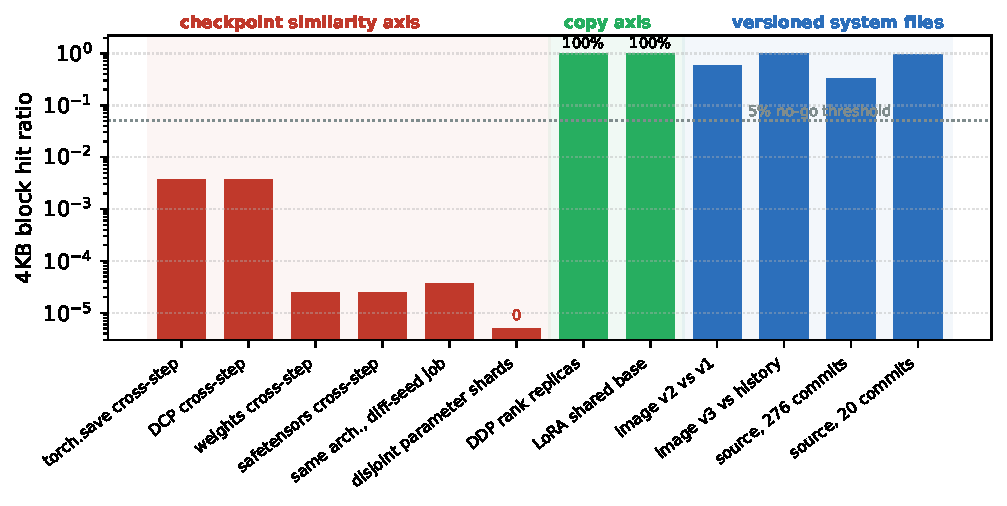
\includegraphics[width=0.66\textwidth]{f1_teaser.pdf}
\caption{Cross-step hit-any ratio per checkpoint format and chunk size
(log scale). The byte layer finds only zero blocks on training
checkpoints (red), versus 59--98\% hits for container image layers and
source archives.}
\label{fig:teaser}
\end{figure*}

\section{Findings}
\label{sec:findings}

\subsection{Temporal redundancy is invisible at the byte layer}

\begin{table}[t]
\caption{Steady-state (steps 5--19) cross-step hit-any ratios. Every hit
is a zero block.}
\label{tab:f1}
\small
\begin{tabular}{lrrrr}
\toprule
\textbf{Layout / view} & \textbf{4\,KB} & \textbf{64\,KB} &
\textbf{1\,MB} & \textbf{4\,MB} \\
\midrule
\texttt{torch.save} / file    & 0.0037 & 0.0036 & \textbf{0.0014} & 0 \\
\texttt{torch.save} / zipdata & 0.0037 & 0.0037 & 0.0029 & 0 \\
weights-only / file           & 0      & 0      & \textbf{0}      & 0 \\
DCP / file                    & 0.0037 & 0.0036 & 0.0028 & 0 \\
\bottomrule
\end{tabular}
\end{table}

Every hit in the full-checkpoint rows
(Table~\ref{tab:f1}, Figure~\ref{fig:teaser}) is an all-zero block:
exact-block ratio equals zero-block ratio (0.37\%), and weights-only
files score exactly zero at every size. At 1\,MB, all-pairs Jaccard
across steps 0--19 is a flat 0.000351 regardless of step distance.
Temporal similarity---what AdaCheck and AITURBO harvest step after
step---does not exist as equal bytes. Notably, AITURBO's finest
detection granularity is 4\,MB~\cite{aiturbo}; at exactly that setting
every format yields zero cross-step hits---XPU hashing would be spent on
a stream containing nothing to find.

\begin{figure}[t]
\centering
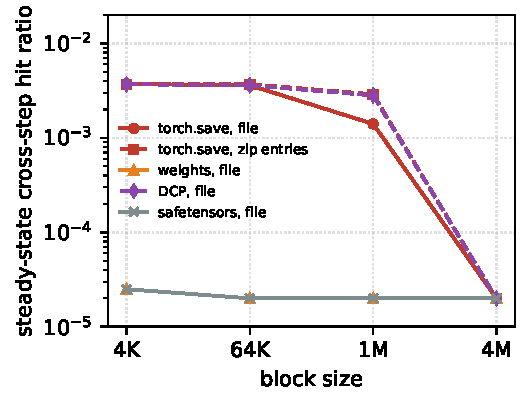
\includegraphics[width=0.82\columnwidth]{f2_chunksizes.pdf}
\caption{Hit-any ratio vs.\ chunk size: no size recovers cross-step
redundancy.}
\label{fig:chunksizes}
\end{figure}

\noindent\textbf{Not an alignment problem.}
Two complementary tests. \emph{Within} checkpoints, shifting the previous
checkpoint's chunk grid by 1, 16, or 256 bytes leaves the hit ratio
unchanged (e.g.\ 0.001404 at 1\,MB for every shift; a 4096 shift removes
the prefix chunk and nothing else). Identical-but-drifting content, the
failure mode content-defined chunking fixes, is absent: there is no hidden
redundancy for CDC to uncover (Figure~\ref{fig:chunksizes}).

\emph{Across} workload families, alignment matters sharply. Chunking
archive byte streams naively (raw tar view) collapses even our positive
controls: rootfs 4\,KB hits drop 58.6\%$\to$3.9\% (v2) and
97.7\%$\to$10.4\% (v3); source archives drop 94.8\%$\to$54.3\% in the
closest pair and to 1.4--4.5\% at moderate distances; at 1\,MB every
raw-stream pair is zero, as tar reordering and headers destroy grid
alignment. Checkpoint zipdata entries, in contrast, \emph{are} chunked
from independent aligned boundaries---and still score zero. Alignment is
necessary (wrong boundaries read zero) but not sufficient.

\begin{figure}[t]
\centering
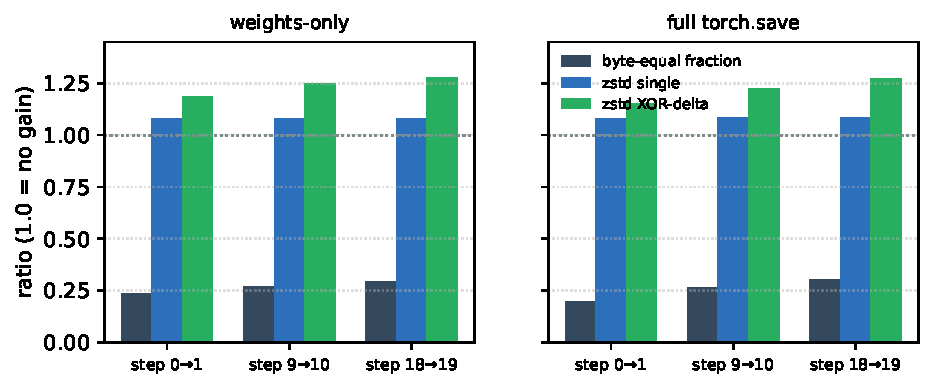
\includegraphics[width=0.88\columnwidth]{f4_delta.pdf}
\caption{Adjacent-step byte equality is only 19.8--30.3\%; zstd and
XOR-delta zstd find almost no redundancy either.}
\label{fig:delta}
\end{figure}

\noindent\textbf{Not precision, age, or compressibility.}
\emph{Precision control.} bf16 weights across 100 steps yield 6--11
matching 4\,KB blocks out of 60,726 ($\le$0.018\%) and zero at 64\,KB or
1\,MB; fp32 weights are exactly zero at gaps of 1, 50, and 100 steps.
Lower mantissa precision does not quantise Adam updates into
byte-identical blocks.

\emph{Format control.} A safetensors run replaying the \textbf{identical}
20-step sequence (bit-identical losses: 10.989, 10.916, 10.968, \dots)
scores 0.0025\% hits at 4\,KB and zero above---the result is a property
of the bytes, not the zip container.

\emph{Compression control.} Perhaps redundancy exists in a form blocks
cannot express (Figure~\ref{fig:delta}). zstd-1 on one checkpoint
compresses 1.08$\times$; an XOR-delta stream between adjacent steps
compresses only 1.15--1.28$\times$; byte-wise equality between adjacent
steps is just 19.8--30.3\%. fp32 training state in motion carries almost
no extractable redundancy by any measure.

\noindent\textbf{Mechanism: every byte is touched every step.}
The zero result has a precise mechanism. (1)~AdamW applies decoupled
weight decay: every participating element receives
$p \leftarrow p - \mathit{lr}\cdot\mathit{wd}\cdot p$ each step, a
relative change of $10^{-5}$---small but guaranteed to flip fp32 low
bytes. (2)~Adam momentum slots decay and accumulate per element.
(3)~In our tied-head GPT-2, the lm-head backward produces a dense
gradient through the whole embedding matrix, and the embedding backward
materialises \textbf{zero (not \texttt{None}) gradients} for unsampled
rows, so weight decay touches those rows too---we verified that rows
unused by the current batch still change bytes every step. At fp32,
essentially every parameter byte changes each step, while tensor
\emph{keys} (names, shapes, identity) stay constant: the whole axis
boundary in one sentence.

\noindent\textbf{Redundancy-axis map: copies visible, similarities invisible.}
\label{sec:axismap}
\begin{table}[t]
\caption{Axis map (per-file aligned blocks, same trained states).}
\label{tab:axismap}
\scriptsize
\setlength{\tabcolsep}{3.5pt}
\begin{tabular}{p{0.95cm}p{2.85cm}rrr}
\toprule
\textbf{Axis} & \textbf{Comparison} & \textbf{4\,KB} &
\textbf{64\,KB} & \textbf{1\,MB} \\
\midrule
A copies & DDP rank replicas (\texttt{torch.save}/safetensors) & 1.000 & 1.000 & 1.000 \\
A divides & Disjoint FSDP/TP shards vs earlier shards & 0 & 0 & 0 \\
B cross-job & full ckpt / weights safetensors, diff.\ seed & 0.000 & 0.000 & 0.0007 \\
B LoRA & shared base file, job2 vs job1 & 1.000 & 1.000 & 1.000 \\
B LoRA & distinct adapter files & 0 & 0 & --- \\
B LoRA & whole-job directories & 0.9988 & 0.9988 & 1.000 \\
C temporal & consecutive steps (Table~\ref{tab:f1}) & 0.0037$^*$ & 0.0036$^*$ & 0--0.0029 \\
\bottomrule
\end{tabular}

\vspace{2pt}
\footnotesize $^*$hits are zero blocks. The single 1\,MB inter-job hit
(1 of 1,423 blocks) is zero content, not structure.
\end{table}

Whole-object copies---rank replicas and shared base files---collapse to
one physical copy transparently; the LoRA directory result (99.9\%)
shows a transparent store already handles the dominant bytes of the LoRA
pattern, missing only the 0.6\,MB adapters. Everything requiring
recognition of ``the same parameter in another version''---consecutive
steps, independent jobs, disjoint shards---is invisible. The
6--896$\times$ headline savings of semantic systems live on this
invisible side; their framework requirements are forced by where the
redundancy is.

\begin{figure}[t]
\centering
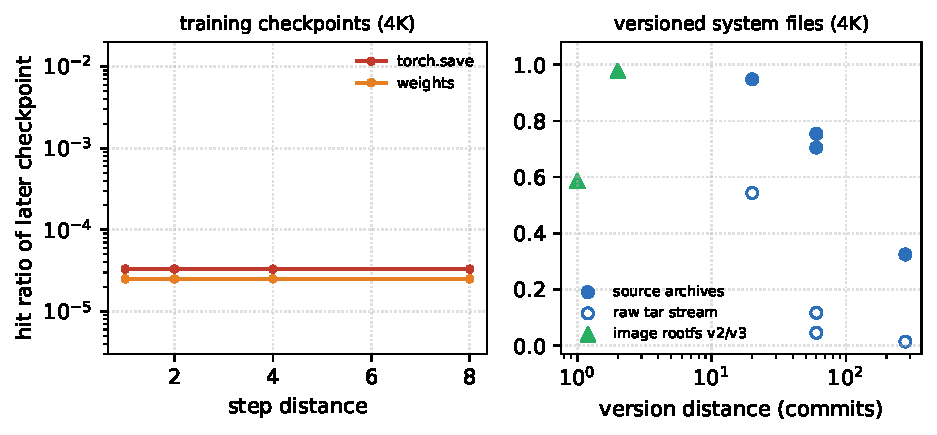
\includegraphics[width=0.88\columnwidth]{f3_distance.pdf}
\caption{Hit ratio vs.\ version distance (log x): checkpoints stay at
the zero-block floor; source/rootfs overlaps stay high.}
\label{fig:distance}
\end{figure}

\noindent\textbf{Positive controls: the same instrument scores 59--98\%.}

\begin{table}[t]
\caption{Positive controls (per-file view, hit-any).}
\label{tab:controls}
\footnotesize
\setlength{\tabcolsep}{4pt}
\begin{tabular}{p{3.55cm}rrr}
\toprule
\textbf{Workload} & \textbf{4\,KB} & \textbf{64\,KB} & \textbf{1\,MB} \\
\midrule
Image rootfs v2 vs v1 & 0.586 & 0.623 & 0.660 \\
Image rootfs v3 vs v1+v2 & \textbf{0.977} & 0.974 & \textbf{0.981} \\
Source, $\sim$276 commits apart & 0.324 & 0.115 & --- \\
Source, moderate gaps & 0.705/0.754 & 0.563/0.585 & --- \\
Source, $\sim$20 commits apart & \textbf{0.948} & \textbf{0.956} & --- \\
Training checkpoints (all formats) & \textbf{0} & 0 & 0 \\
\bottomrule
\end{tabular}
\end{table}

The 75\,MB ubuntu base blob is shared verbatim across all three images;
even the 191/197\,MB sibling application layers---full reinstalls---
contain 59\% and 98\% of blocks seen earlier, because dpkg overwrites the
same library and binary files with identical content
(Table~\ref{tab:controls}, Figure~\ref{fig:distance}). System files are
byte-stable across versions; optimizer state is byte-stable for exactly
one step. With the same code scoring 98\% and 0\%, the zero cannot be
blamed on the instrument.

\section{Implications: Learn to Skip, Not to Deduplicate}
\label{sec:implications}

\textbf{A classifier before the hash.} If hashing is expensive
(AITURBO's XPU is the admission~\cite{aiturbo}) and temporal checkpoints
never hit, a transparent client should not be smarter about \emph{how} it
hashes checkpoint streams---it should decide \emph{whether to hash at
all}, from signals available before touching bytes: write pattern
(periodic large sequential file from a training job), file size/age,
directory topology (rank replicas), and cheap prefix probes. Copy-heavy
paths (rank replicas, base models, image pulls, log/tar bundles) always
hash; churn-heavy training state skips to write-through.

\textbf{Asymmetric loss keeps ML off the correctness path.} A gating
classifier makes one mistake in each direction: a false positive (hashed
a unique stream) wastes fingerprints; a false negative (skipped a
redundant stream) loses one saving. Both affect performance only.
Suppression still requires an exact fingerprint match, so ML can neither
corrupt data nor lose a byte---unlike prediction-in-the-data-path
systems such as LinnOS~\cite{linnos} or KML's learned kernel
heuristics~\cite{kml}: prediction proposes, exact matching disposes. Our
measurements supply the labelled \textbf{negative} workloads such a gate
previously lacked; earlier write-side prediction only knew workloads
where redundancy is the default.

\textbf{A lower bound, not an obituary, for semantic systems.} The zero
on the similarity axis quantifies the \emph{necessity} of tensor
cooperation: no transparent cleverness---CDC, larger blocks,
compression---can intercept savings whose identical units are tensor
keys, not bytes. The 100\% on the copy axis, conversely, shows
transparent dedup remains right for replicated saves and shared bases; a
deployed system should compose both.

\textbf{Existence proof.} In our research POSIX filesystem, an inline
kernel content-hash fast path with a gated write needle cuts dedup
metadata RPCs from 1,024 to 258 per 256\,MB write round and improves
steady-state write bandwidth by 50\% across four rounds, with
md5-identical output. The gated path is cheap and safe; this paper
determines \emph{where it must not be switched on}. (System name
withheld for blind review.)

\section{Related Work}
\label{sec:related}

\textbf{Semantic checkpoint storage.} AdaCheck~\cite{adacheck} rewrites
tensors across parallelism, architecture, and temporal dimensions;
AITURBO~\cite{aiturbo} adds grouped I/O and XPU BLAKE3 fingerprinting.
Kaiser et al.~\cite{kaiser2016}, the closest predecessor, measured
byte-level deduplication potential across HPC checkpoints, where static
memory regions produced application-dependent savings. We revisit the
question for AI-training state under AdamW, splitting redundancy into
copy and similarity axes: the answer flips for temporal similarity but
holds for copies.

\textbf{Block deduplication and chunking.} Venti~\cite{venti}
established content-addressed blocks; iDedup~\cite{idedup} studied inline
deduplication and its fragmentation cost; LBFS~\cite{lbfs} introduced and
FastCDC~\cite{fastcdc} optimised content-defined chunking. Our shift
sweep tests CDC's precondition (offset-drifted identical content) directly
and finds it absent.

\textbf{Learning in storage.} LinnOS~\cite{linnos} reroutes I/Os from a
learned latency model; KML~\cite{kml} sets kernel heuristics such as
readahead with learned models. In both, model output directly changes the
I/O action. Our gate differs structurally: ML decides only whether an
exact algorithm runs, never what data it returns.

\textbf{AI storage workloads.} Mooncake~\cite{mooncake} accelerated
KVCache-centric serving traffic, a separate track we do not enter.
Traditional-workload baselines (FIU/MSR traces) are deferred to the
full-paper version.

\section{Limitations and Conclusion}
\label{sec:limitations}

\textbf{Limitations.} One architecture (124\,M GPT-2), one optimiser
family (AdamW), random-token training, CPU, and single-process fixtures:
absolute numbers will move at scale, but the mechanism (per-element
updates flip fp32 bytes; similarity keys are tensor names) is
architecture-independent, and our controls isolate it directly.
Multi-node traces, non-AdamW optimisers, and a full CDC implementation
(we give strong precondition evidence rather than an implementation) are
clear extensions, as are read-side fragmentation effects on restore.

\textbf{Conclusion.} Redundancy splits sharply at the POSIX boundary: the
byte layer sees every \emph{copy} (100\%) and nearly none of the
\emph{similarity} ($\approx$0\%) semantic systems monetise, while the
same code scores 59--98\% on images and sources. Transparent storage
cannot earn that 6--896$\times$; it should learn to skip churn and
reserve exact fingerprinting for where copies live.

% Acknowledgments: camera-ready only (double-blind submission).

\bibliographystyle{ACM-Reference-Format}
\bibliography{refs}

\end{document}
\endinput
